\documentclass[12pt,a4paper]{article}

\usepackage[utf8]{inputenc}
\usepackage[T1]{fontenc}
\usepackage[francais]{babel}
\usepackage{setspace}
\usepackage{graphicx}

\title{Diagramme d'architecture}

\author{Hereiti \bsc{Hatitio} - Anta \bsc{Mbaye} - Maxime \bsc{Vincent} - Jean-Baptiste \bsc{Rey}}

\begin{document}
\maketitle

\newpage
\vspace*{-1.6in}
\vspace*{-\the\hoffset}
\thispagestyle{empty}
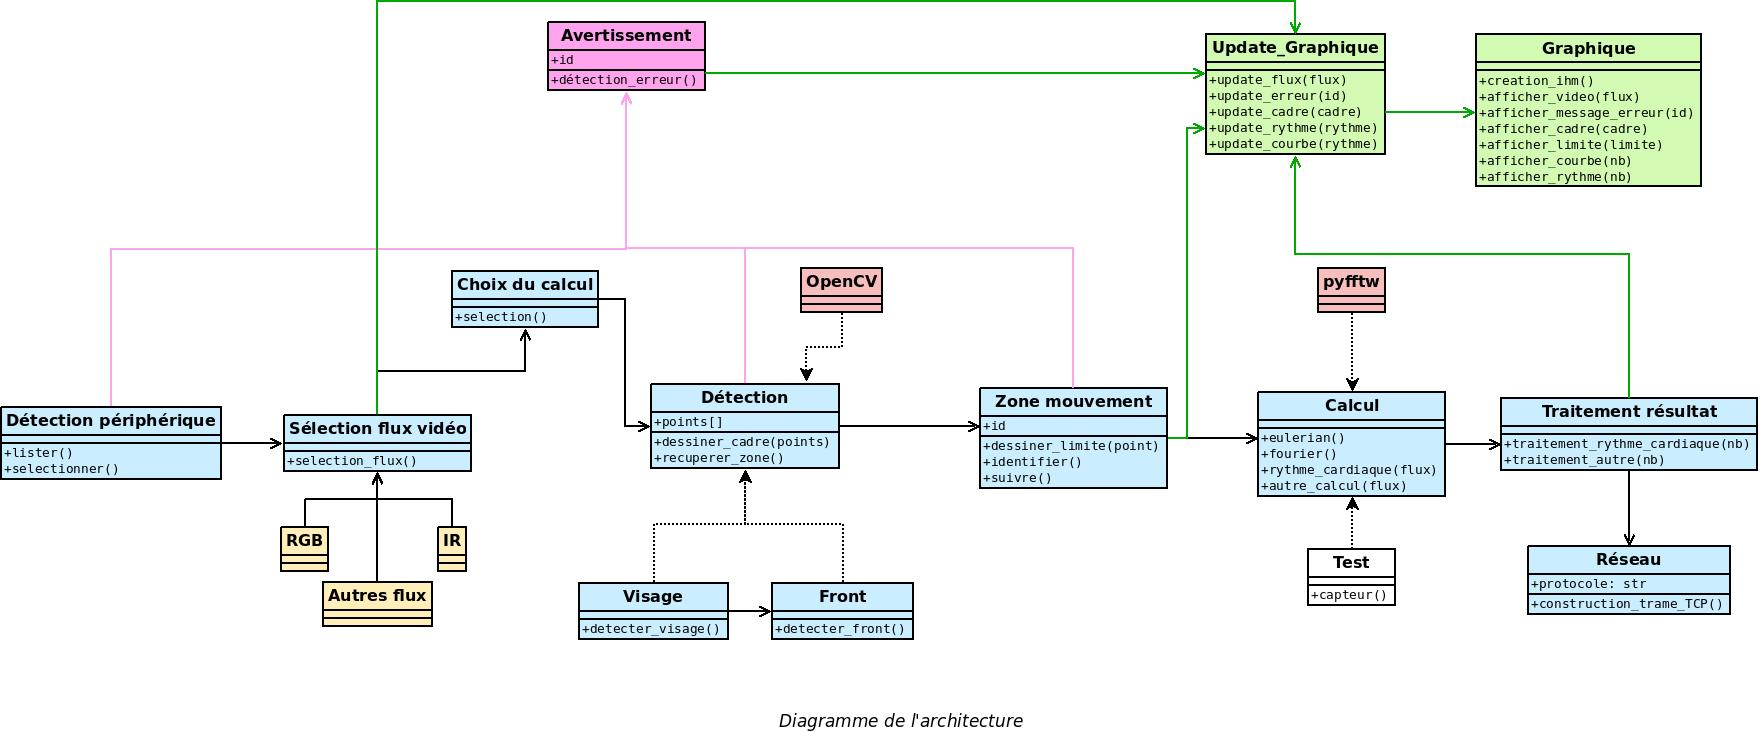
\includegraphics[scale=0.4,angle=90]{archi2.jpeg}
\begin{center}

\end{center}
\vspace*{-1in}
\vspace*{-\the\hoffset}

\includegraphics[scale=0.5]{bleu.png} : Modules implémentant les besoins fonctionnels\newline
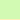
\includegraphics[scale=0.5]{vert.png} : Modules d'affichage graphique\newline

\includegraphics[scale=0.5]{orange.png} : Flux vidéo\newline

\includegraphics[scale=0.5]{rouge.png} : Frameworks\newline

\includegraphics[scale=0.5]{rose.png} :  Module de traitement des erreurs\newline
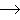
\includegraphics[scale=0.5]{fleche.png} :  Implémentation\newline
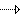
\includegraphics[scale=0.5]{fleche_pointille.png} :  Transitions\newline
\section*{Modules}

\subsection*{Détection périphériques}
Ce module liste les différents périphériques utilisables. Il permet à l'utilisateur d'en sélectionner un.

\subsection*{Sélection flux vidéo}

Ce module permet de sélectionner le flux (RGB, IR ou autres) pour appliquer le tracking. Le flux sera ensuite affiché dans l'IHM.

\subsection*{Choix du calcul}
Ce module permet la sélection du type de mesure physiologique. Dans notre cas le rythme cardiaque, avec possibilité de rajouter le calcul du rythme respiratoire ou autre.

\subsection*{Détection}
A l'aide d'OpenCV, ce module permet de détecter la zone de traitement suivant un choix de l'utilisateur, puis de dessiner le cadre de cette zone.

\subsection*{Visage}
Ce module permet d'isoler un visage à partir du flux vidéo.

\subsection*{Front}
Ce module isole le front à partir de la zone calculée par le module \textit{Visage}

\subsection*{Zone mouvement}

Ce module délimite la zone de mouvement possible sans perte de tracking. Il identifie également les utilisateurs par un ID numérique. Si un utilisateur sort de son cadre, le tracking est perdu, il n'est repris que lorsqu'une nouvelle zone de traitement est détectée.

\vspace*{-1.01in}

\subsection*{Calcul}

Ce module effectue le calcul sélectionné dans \textit{Choix du calcul}. Il mesure en boucle le rythme cardiaque tant qu'une zone de traitement est valide.
Le même algorithme est appliqué sur chaque sujet détecté.\newline
\textit{pyfftw} est utilisé pour implémenter l'algorithme basé sur les transformés de Fourier.

\subsection*{Traitement résultat}
Ce module récupère les résultats fournis par \textit{Calcul} et les rend compatible avec les modules \textit{Update\_Graphique} et \textit{Réseau}.

\subsection*{Réseau}
Ce module encapsule les données de \textit{Traitement résultat} au sein de trames TCP prêtes à être envoyées vers un serveur client.
Il utilisera des protocoles de types OSC et LSL.

\subsection*{Avertissements}
En cas d'erreurs produites par les différents modules précédents, un message est envoyé au module \textit{Update\_graphique} qui met à jour l'IHM en spécifiant l'erreur.

\subsection*{Update\_graphique}
Ce module correspond à un \textit{Listener}. Il permet de mettre à jour les différents éléments de l'interface graphique.

\subsection*{Graphique}
Ce module affiche les différents éléments composant de l'IHM.
\newpage
\section*{Test}
Ce module compare les données calculées via le flux vidéo avec celles d'un capteur de contact (capteur Arduino).

\section*{Framework}
\textit{OpenCV} et \textit{pyfftw} sont des bibliothèques qui sont utilisées respectivement par les modules \textit{Détection} et \textit{Calcul}.


\end{document}